\documentclass[dvipdfmx,autodetect-engine,titlepage]{jsarticle}
\usepackage[dvipdfm]{graphicx}
\usepackage{ascmac}
\usepackage{fancybox}
\usepackage{listings}
\usepackage{plistings}
\usepackage{itembkbx}
\usepackage{amsmath}
\usepackage{svg}
\usepackage{url}
\usepackage{graphics}
\usepackage{listings,jvlisting}

\textheight=23cm
\renewcommand{\figurename}{図}
\renewcommand{\tablename}{表}
\newenvironment{code}
{\vspace{0.5zw}\VerbatimEnvironment  
\begin{screen} 
\baselineskip=1.0\normalbaselineskip
 \begin{Verbatim}}
{\end{Verbatim}
\baselineskip=\normalbaselineskip
 \end{screen}\vspace{0.5zw}} 

\title{情報理工学部 SNコース 3回\\
Cプログラム脆弱性実習レポート\\}
\author{2600200443-6\\Yamashita Kyohei\\山下 恭平}
\date{Apr 25 2021}

\begin{document}

\maketitle

\section{問1}

\subsection{解答}

入力文字に「Sophisticated」と入力した。その結果を図1に示す。

\begin{figure}[h]
  \centering
  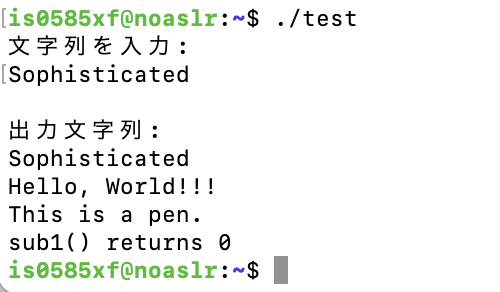
\includegraphics[scale=1]{pic1.png}
  \caption{出力結果}
\end{figure}

\section{問2}

\subsection{解答}

「\%E5\%B1\%B1\%E4\%B8\%8B\%E6\%81\%AD\%E5\%B9\%B3」と入力し、
出力として「山下恭平」を得た。その結果を図2に示す。

\begin{figure}[h]
  \centering
  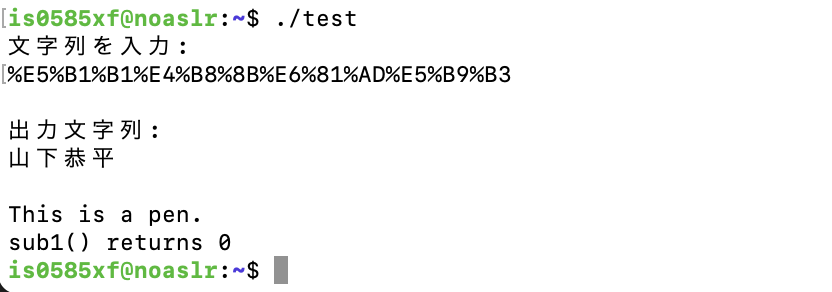
\includegraphics[scale=1]{pic2.png}
  \caption{出力結果}
\end{figure}

\subsection{解説}
GCCでプログラムをコンパイルするとき、文字列はUTF-8でコンパイルされるので、
直接メモリ上にUTF-8の文字コードを入力することで実現した。

\section{問3}

\subsection{解答}
入力に「01234567890123456789012345678901Ritsumeikan」と与え、
題意を満たす出力を得た。その結果を図3に示す。

\begin{figure}[h]
  \centering
  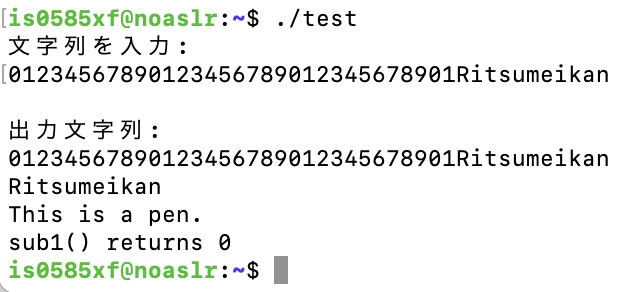
\includegraphics[scale=1]{pic3.png}
  \caption{出力結果}
\end{figure}

\section{問4}

\subsection{解答}

入力に「01234567890123456789012345678901Ritsumeikan12345\%38\%40\%40」と与え、題意を満たす出力を得た。その結果を図4に示す。
\begin{figure}[h]
  \centering
  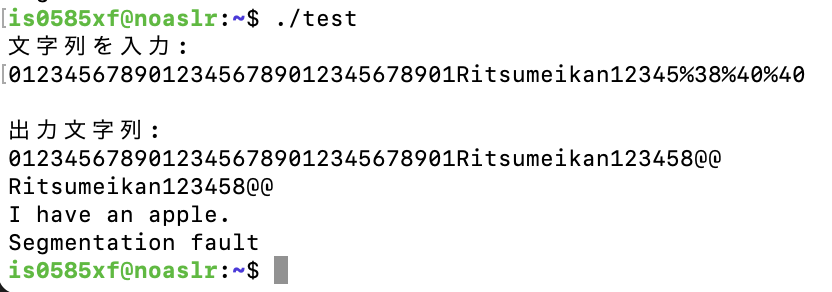
\includegraphics[scale=1]{pic4.png}
  \caption{出力結果}
\end{figure}

\section{問5}

\subsection{解答}

入力に「01234567890123456789012345678901Ritsumeikan12345\%28\%40\%40\%00\%00\%40\%40\%00\%00\\\%10\%fc\%b7\%18\%f6\%ff\%bf\%c9\%11\%40」
と与え、題意を満たす出力を得た。その結果を図5に示す。

\begin{figure}[h]
  \centering
  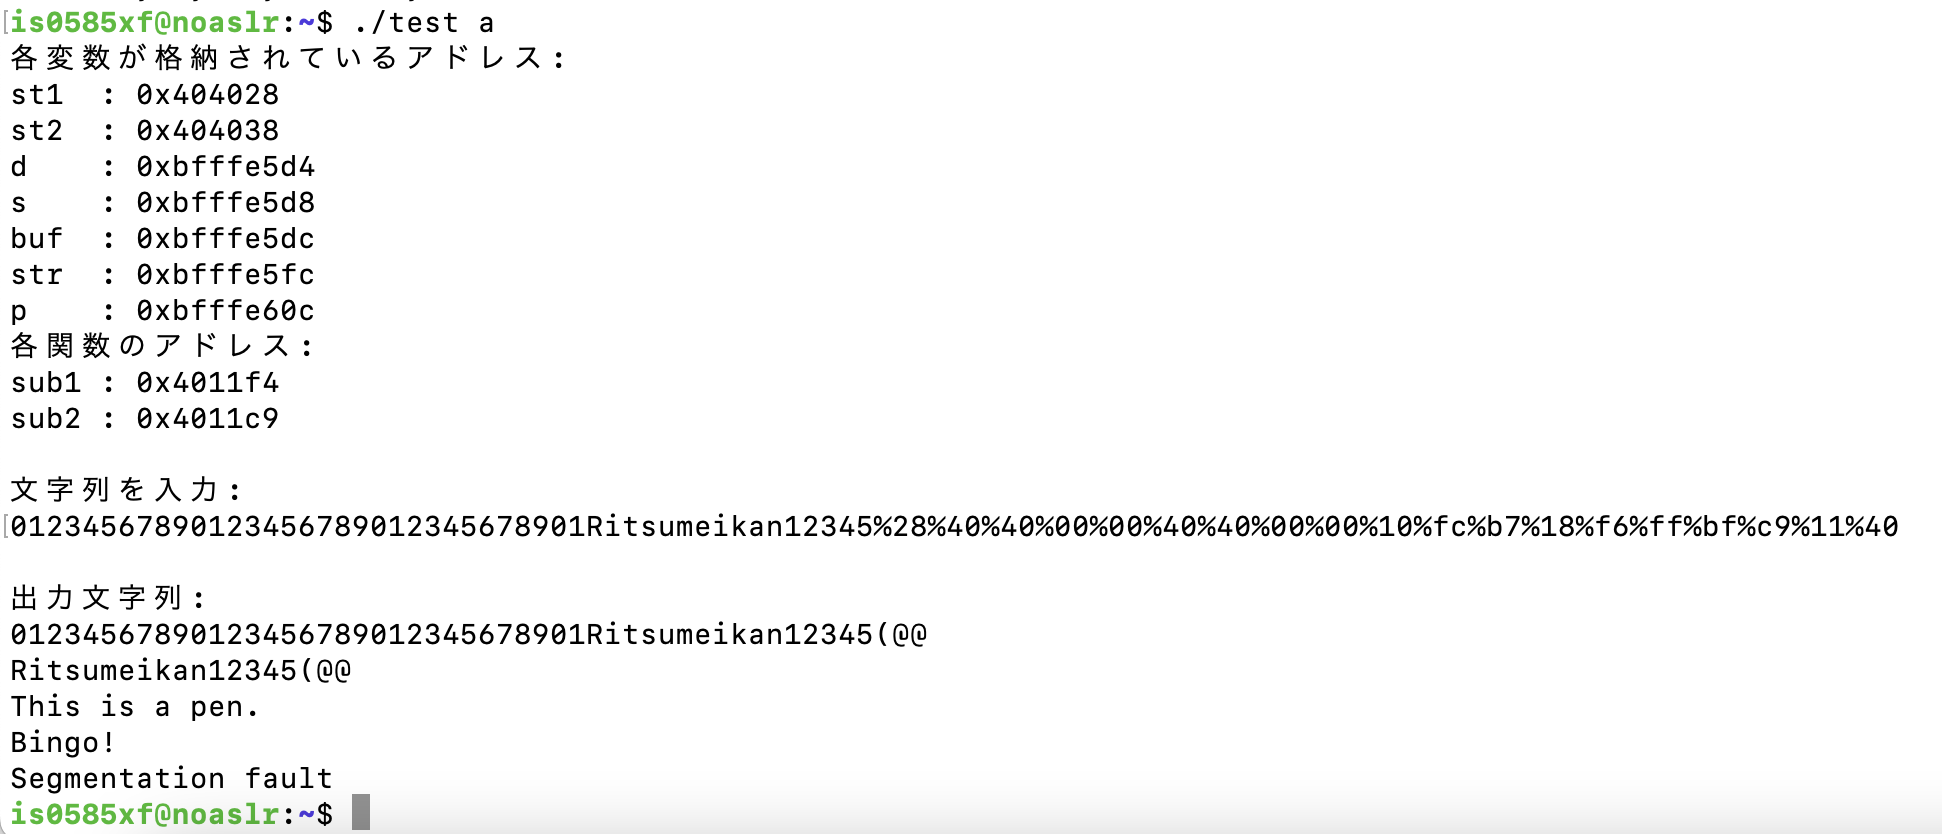
\includegraphics[scale=0.45]{pic5.png}
  \caption{出力結果}
\end{figure}

\subsection{解説}
testをgdbを用いてデバッグを行った。初めにメイン関数をディスアセンブリし、
戻りアドレスを特定した。(図6)

\begin{figure}[h]
  \centering
  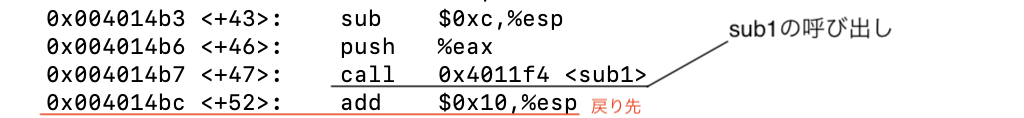
\includegraphics[scale=1]{pic6.png}
  \caption{出力結果}
\end{figure}

次に、bufを先頭に108バイト分のメモリの内容を表示し、
戻りアドレス「0x004014bc」がeip(0xbfffe5ec)に格納されているのを確認する。
この時IntelCPUはリトルエンディアンであるので、メモリには下位ビットである
「bc」から格納されていることに気をつける。(次ページ図7)

書き換えるアドレスを特定したので、オーバーフローを起こし書き換えていくが、
リターン実行前にセグメンテーションフォルトを起こしてはいけないので、buf,strの外
側ではあらかじめメモリに格納されていたアドレスを格納していき、戻りアドレスだけを
書き換える必要がある。

\begin{figure}[htbp]
  \centering
  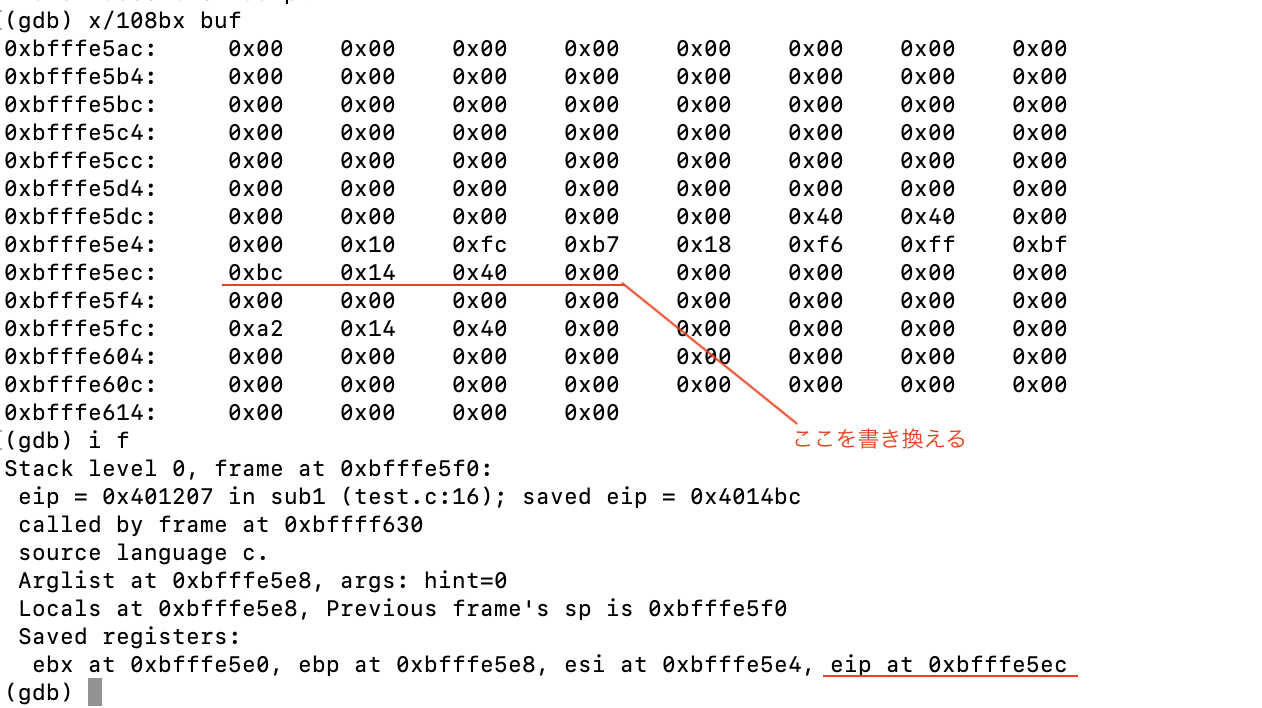
\includegraphics[scale=0.8]{pic7.png}
  \caption{出力結果}
\end{figure}


\end{document}

